\documentclass{elegantpaper}
\usepackage{amsmath, amssymb, booktabs, amsthm}

\title{MATH 4665 Homework 4}
\author{Jiahan XIA}
\makeatletter
\let\@date\empty
\makeatother

\begin{document}
\maketitle

\section*{Question 1: Existence and Uniqueness of PDE Solutions}

\subsection*{(a) Formulation in a Sobolev space}

Consider the one-dimensional Poisson equation with Dirichlet boundary conditions:
\begin{equation}
    -u''(x) = f(x), \quad x \in (0,1), \quad u(0) = u(1) = 0.
\end{equation}
To derive the weak formulation, we multiply the strong form by a smooth test function $v \in C_c^\infty(0,1)$ and integrate over the domain $(0,1)$:
\begin{equation}
    -\int_0^1 u''(x)v(x) \, dx = \int_0^1 f(x)v(x) \, dx.
\end{equation}
Applying integration by parts to the left-hand side, we obtain:
\begin{equation}
    - \left[ u'(x)v(x) \right]_0^1 + \int_0^1 u'(x)v'(x) \, dx = \int_0^1 f(x)v(x) \, dx.
\end{equation}
Since $v$ vanishes at the boundary ($v(0) = v(1) = 0$), the boundary term drops out. The weak formulation is: find $u \in V$ such that
\begin{equation}
    a(u,v) = L(v) \quad \forall v \in V,
\end{equation}
where the bilinear form $a(\cdot, \cdot)$ and the linear functional $L(\cdot)$ are defined as:
\begin{equation}
    a(u,v) = \int_0^1 u'(x)v'(x) \, dx, \quad L(v) = \int_0^1 f(x)v(x) \, dx.
\end{equation}

\paragraph{Function spaces:}
The function space $V$ containing the weak-form solution $u$ and the class of test functions $v$ is the Sobolev space $H_0^1(0,1)$, which is the closure of $C_c^\infty(0,1)$ with respect to the $H^1$-norm. It consists of functions in $L^2(0,1)$ with weak derivatives in $L^2(0,1)$ and zero trace on the boundary. The norm is $\|u\|_{H^1} = \left( \|u\|_{L^2}^2 + \|u'\|_{L^2}^2 \right)^{1/2}$.

\paragraph{Continuity and Coercivity assumptions:}
For the bilinear form $a(u,v)$ to be continuous, we need a constant $M > 0$ such that $|a(u,v)| \le M \|u\|_V \|v\|_V$. By the Cauchy-Schwarz inequality in $L^2$, we have:
\begin{equation}
    |a(u,v)| \le \int_0^1 |u'(x)v'(x)| \, dx \le \|u'\|_{L^2} \|v'\|_{L^2} \le \|u\|_{H^1} \|v\|_{H^1}.
\end{equation}
Thus, $a(u,v)$ is continuous with $M = 1$.

For coercivity, we need a constant $\alpha > 0$ such that $a(u,u) \ge \alpha \|u\|_V^2$. This relies on the \textbf{Poincar\'e inequality}, which states that for $u \in H_0^1(0,1)$, there exists a constant $C_P > 0$ such that $\|u\|_{L^2} \le C_P \|u'\|_{L^2}$. Consequently,
\begin{equation}
    \|u\|_{H^1}^2 = \|u\|_{L^2}^2 + \|u'\|_{L^2}^2 \le (C_P^2 + 1) \|u'\|_{L^2}^2 = (C_P^2 + 1) a(u,u).
\end{equation}
Therefore, $a(u,u) \ge \frac{1}{C_P^2 + 1} \|u\|_{H^1}^2$, establishing coercivity with $\alpha = 1/(C_P^2 + 1)$.

\subsection*{(b) Lax--Milgram theorem and Application}

\paragraph{Lax--Milgram Theorem:} Let $V$ be a real Hilbert space. Let $a: V \times V \to \mathbb{R}$ be a bilinear form that is continuous and coercive. Let $L: V \to \mathbb{R}$ be a continuous linear functional. Then, there exists a unique element $u \in V$ such that $a(u,v) = L(v)$ for all $v \in V$.

\paragraph{Proof Idea:} 
By the Riesz Representation Theorem, the continuous linear functional $L(v)$ can be uniquely represented as $L(v) = \langle w, v \rangle_V$ for some $w \in V$. Similarly, for a fixed $u \in V$, the map $v \mapsto a(u,v)$ is a continuous linear functional, so there exists a unique element $Au \in V$ such that $a(u,v) = \langle Au, v \rangle_V$. The operator $A: V \to V$ is linear and bounded. The problem reduces to finding $u \in V$ such that $Au = w$.

\begin{itemize}
    \item \textbf{Uniqueness (Injectivity):} Coercivity implies $\alpha \|u\|_V^2 \le a(u,u) = \langle Au, u \rangle_V \le \|Au\|_V \|u\|_V$, so $\|Au\|_V \ge \alpha \|u\|_V$. If $Au_1 = Au_2$, then $\|A(u_1 - u_2)\|_V \ge \alpha \|u_1 - u_2\|_V \implies 0 \ge \alpha \|u_1 - u_2\|_V \implies u_1 = u_2$, so $A$ is injective. This bounded-below property also ensures that the range of $A$, denoted $R(A)$, is closed.
    \item \textbf{Existence (Surjectivity):} To show a solution exists for any $L$, we must prove $R(A) = V$. Since $R(A)$ is closed, if $R(A) \neq V$, there would exist a non-zero $z \in V$ orthogonal to $R(A)$. This means $\langle Au, z \rangle_V = 0$ for all $u \in V$. Choosing $u = z$, we get $\langle Az, z \rangle_V = a(z,z) = 0$. However, coercivity requires $a(z,z) \ge \alpha \|z\|_V^2 > 0$ for $z \neq 0$, which is a contradiction. Thus, $R(A) = V$, meaning $A$ is surjective. Therefore, for our specific $w \in V$, there exists a $u \in V$ such that $Au = w$.
\end{itemize}
Since $A$ is both injective and surjective (a bijection), $u = A^{-1}w$ is the unique solution.

\paragraph{Application to the Poisson Problem:}
As established in part (a), $V = H_0^1(0,1)$ is a Hilbert space. The bilinear form $a(u,v) = \int_0^1 u'v' \, dx$ is continuous and coercive. Assuming $f \in L^2(0,1)$, the linear functional $L(v) = \int_0^1 fv \, dx$ is continuous because:
\begin{equation}
    |L(v)| \le \|f\|_{L^2} \|v\|_{L^2} \le \|f\|_{L^2} \|v\|_{H^1}.
\end{equation}
Since all hypotheses of the Lax--Milgram theorem are satisfied, there exists a unique weak solution $u \in H_0^1(0,1)$ to the 1D Poisson equation.

\newpage
\section*{Question 2: Kernel Ridge Regression (KRR)}

\subsection*{(a) The Representer Theorem and Linear System}

The core challenge in this section is showing how an optimization problem over an infinite-dimensional space $\mathcal{H}_k$ collapses into a finite-dimensional one.

\subsubsection*{1. Applying the Representer Theorem}

The Representer Theorem states that for a loss function and a strictly increasing regularization term, the minimizer $\hat{f}_{n,\lambda}$ must lie in the span of the kernel functions evaluated at the data points.

\begin{itemize}
    \item \textbf{The Logic:} Any function $f \in \mathcal{H}_k$ can be decomposed into $f = f_{\parallel} + f_{\perp}$, where $f_{\parallel}$ is in the subspace $V = \text{span}\{k(\cdot, X_1), \dots, k(\cdot, X_n)\}$ and $f_{\perp}$ is orthogonal to it.
    \item \textbf{The Reproducing Property:} By the reproducing property, $f(X_i) = \langle f, k(\cdot, X_i) \rangle_{\mathcal{H}_k}$. Since $k(\cdot, X_i) \in V$, the orthogonal component $f_{\perp}$ does not affect the value of $f(X_i)$.
    \item \textbf{The Minimization:} However, $\|f\|_{\mathcal{H}_k}^2 = \|f_{\parallel}\|_{\mathcal{H}_k}^2 + \|f_{\perp}\|_{\mathcal{H}_k}^2$. To minimize the functional, we must set $f_{\perp} = 0$.
    \item \textbf{The Expansion:} Thus, the solution takes the form:
    \begin{equation}
        \hat{f}_{n,\lambda}(x) = \sum_{i=1}^{n} \alpha_i k(x, X_i)
    \end{equation}
\end{itemize}

\subsubsection*{2. Deriving the Linear System}

We substitute the expansion $\hat{f}_{n,\lambda}(x) = \sum_{j=1}^n \alpha_j k(x, X_j)$ back into the regularized least-squares functional.

\begin{itemize}
    \item Define the Kernel Matrix $K \in \mathbb{R}^{n \times n}$ where $K_{ij} = k(X_i, X_j)$.
    \item The vector of predictions is $K\alpha$, and the regularization term becomes $\lambda \alpha^\top K \alpha$.
    \item The objective function in terms of $\alpha$ is:
    \begin{equation}
        J(\alpha) = \frac{1}{n} \|Y - K\alpha\|^2 + \lambda \alpha^\top K \alpha
    \end{equation}
    \item Taking the gradient with respect to $\alpha$ and setting it to zero yields the linear system:
    \begin{equation}
        (K + n\lambda I)\alpha = Y
    \end{equation}
\end{itemize}

\subsection*{(b) Convergence and the Role of $\lambda$}

We outline why the expected squared prediction error $R_n$ goes to zero as $n \to \infty$.

\subsubsection*{1. Proof Outline for Convergence}

\begin{itemize}
    \item \textbf{Operator Framework:} The problem is often analyzed using the Kernel Integral Operator $T_k$. The KRR estimator can be viewed as a filtered version of the true function $f_0$, where the filter is determined by the eigenvalues of $T_k$ and the parameter $\lambda$.
    \item \textbf{Error Decomposition:} The risk $R_n$ is decomposed into two terms:
    \begin{itemize}
        \item \textbf{Approximation Error (Bias):} How well $f \in \mathcal{H}_k$ can represent $f_0$. If $f_0 \in \mathcal{H}_k$, this term vanishes as $\lambda \to 0$.
        \item \textbf{Estimation Error (Variance):} The error introduced by the noise $\epsilon_i$ in the samples.
    \end{itemize}
\end{itemize}

\subsubsection*{2. The Role of the Regularization Parameter $\lambda_n$}

The parameter $\lambda$ acts as a "damper" on the noise.

\begin{itemize}
    \item \textbf{If $\lambda$ is too large:} The model is too simple (high bias), failing to capture the underlying $f_0$.
    \item \textbf{If $\lambda$ is too small:} The model "overfits" the noise $\epsilon_i$ (high variance).
    \item \textbf{For Convergence:} To ensure $R_n \to 0$, we require $\lambda_n \to 0$ as $n \to \infty$, but it must go to zero slowly enough (specifically, $n\lambda_n \to \infty$) so that the noise is averaged out.
\end{itemize}

\subsubsection*{1D KRR Example Illustration}

Below is a 1D KRR example generating data from $f_0(x) = \sin(2\pi x)$ with Gaussian noise. It shows the KRR fit for three different $\lambda$ values to illustrate the bias-variance tradeoff:

\begin{figure}[h]
    \centering
    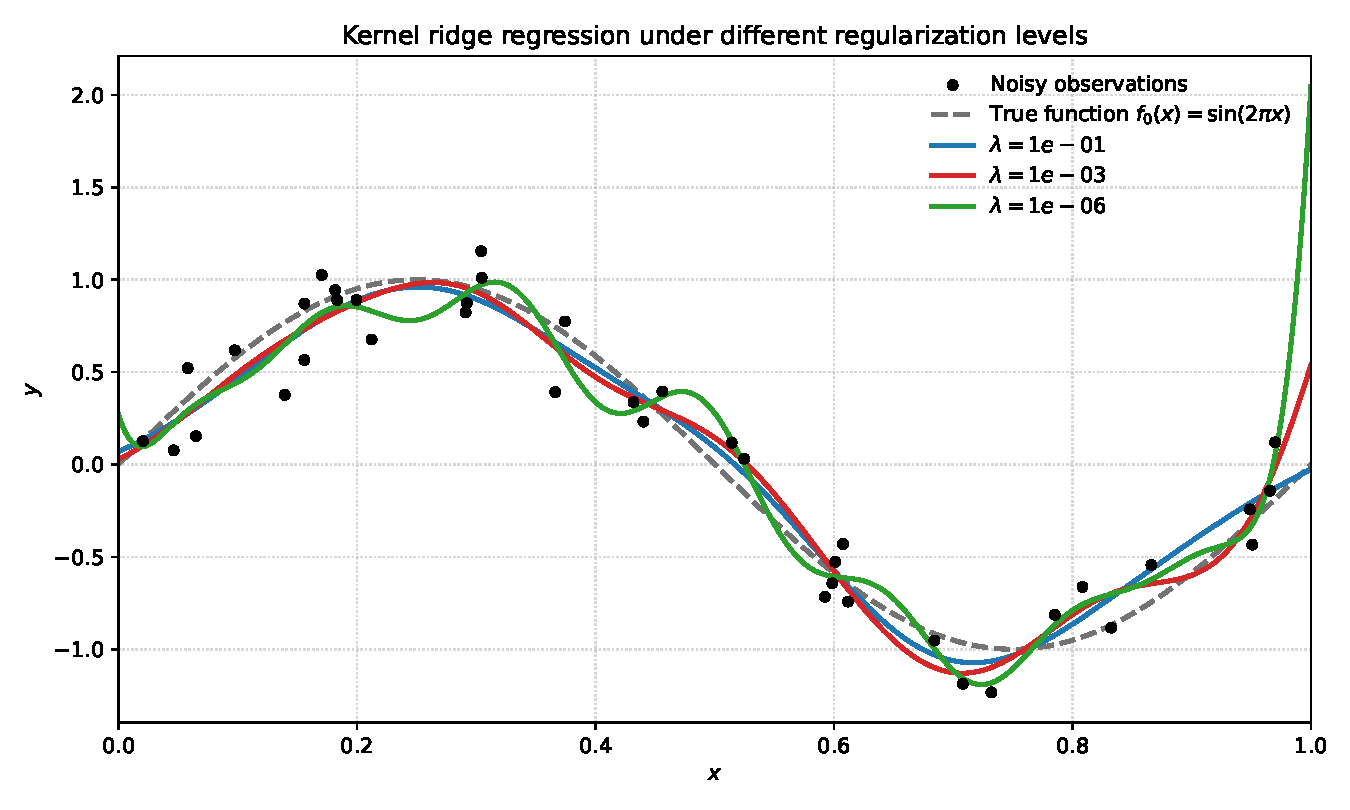
\includegraphics[width=0.8\textwidth]{krr_plot.pdf}
    \caption{1D KRR Example with Gaussian noise. Observation: $\lambda=10^{-1}$ is too smooth (underfit), failing to capture the peak and trough of the sine wave. $\lambda=10^{-8}$ is too wiggly (overfit), matching the noise in the samples. $\lambda=10^{-4}$ provides a good balance, capturing $f_0(x)$ without overfitting the noise, illustrating the balance discussed in 2(b).}
    \label{fig:krr}
\end{figure}

\newpage
\section*{Question 3: Minimax Convergence Rate for KRR}

This section focuses on the fundamental limits of how well any algorithm can perform (Minimax Risk) and how Kernel Ridge Regression (KRR) specifically balances its errors to reach those limits.

\subsection*{(a) Understanding Minimax Risk}

The minimax risk $R_n^*$ represents the "best of the worst" scenario in statistical estimation:
\begin{equation}
    R_n^* = \inf_{\hat{f}_n} \sup_{f_0 \in \Theta} \mathcal{R}_n(\hat{f}_n, f_0).
\end{equation}

\begin{itemize}
    \item \textbf{Parameter Space ($\Theta$):} This is "Nature's choice". It defines the set of all possible true functions $f_0$ that the environment might use to generate the data. Usually, this is a ball in the RKHS, $\Theta = \{f \in \mathcal{H}_k : \|f\|_{\mathcal{H}_k} \le C\}$.
    \item \textbf{The Loss Function:} This is the metric used to evaluate how far the estimate $\hat{f}_n$ is from the truth $f_0$. In this problem, it is the expected $L^2(\mu)$ squared error.
    \item \textbf{The Supremum ($\sup_{f_0 \in \Theta}$):} This identifies the "worst-case" performance of a specific estimator over the entire model class $\Theta$. It ensures our theoretical guarantees hold even for the most difficult functions in our set.
    \item \textbf{The Infimum ($\inf_{\hat{f}_n}$):} This is the statistician's move. We search for the best possible algorithm (the one that minimizes the worst-case error).
    \item \textbf{Theoretical Benchmark:} $R_n^*$ serves as a benchmark because it tells us the absolute limit of performance for a given sample size $n$ and smoothness class $\Theta$. No algorithm can consistently beat this rate for all functions in the class.
\end{itemize}

\subsection*{(b) Mean-Square Error (MSE) Decomposition}

To understand how KRR behaves, we decompose the risk into its variance and bias components.

\subsubsection*{1. The Decomposition}

For a fixed design, the expected risk $R_n$ can be broken down:
\begin{equation}
    \mathcal{R}_n(\hat{f}_{n,\lambda}, f_0) = \underbrace{\mathbb{E}[\|\hat{f}_{n,\lambda} - \mathbb{E}[\hat{f}_{n,\lambda}]\|^2]}_{\text{Variance}} + \underbrace{\|\mathbb{E}[\hat{f}_{n,\lambda}] - f_0\|^2}_{\text{Bias}^2}
\end{equation}

\begin{itemize}
    \item \textbf{Random Quantities:} The noise $\varepsilon_i$ in the labels $Y_i$ and the random sampling of the design points $X_i$.
    \item \textbf{Fixed Quantities:} The true function $f_0$, the kernel $k$, and the regularization parameter $\lambda$.
\end{itemize}

\subsubsection*{2. Balancing with $\lambda_n$}

The parameter $\lambda$ controls the trade-off between bias and variance:
\begin{itemize}
    \item \textbf{Bias:} Increases as $\lambda$ increases because the regularizer "pulls" the solution toward zero, away from the complex $f_0$.
    \item \textbf{Variance:} Decreases as $\lambda$ increases because the regularizer smooths out the fluctuations caused by the random noise $\varepsilon$.
    \item \textbf{The Goal:} As $n \to \infty$, we choose a sequence $\lambda_n$ that shrinks to zero at a specific rate to make both terms vanish simultaneously, optimally balancing the bias and variance to achieve the minimax rate.
\end{itemize}

\end{document}